% THIS DOCUMENT IS FOLLOWS THE VOLERE TEMPLATE BY Suzanne Robertson and James Robertson
% ONLY THE SECTION HEADINGS ARE PROVIDED
%
% Initial draft from https://github.com/Dieblich/volere
%
% Risks are removed because they are covered by the Hazard Analysis
\documentclass[12pt]{article}

% ----- Requirements formatting helpers -----
\usepackage{enumitem}

% A tidy description-style list for requirements
\newlist{reqlist}{description}{1}
\setlist[reqlist]{%
	style=nextline,
	leftmargin=3.2cm,
	labelsep=0.6cm,
	font=\normalfont\bfseries
}

% Inline helpers for rationale/fit criterion
\newcommand{\rationale}[1]{\par\emph{Rationale:} #1}
\newcommand{\fitcrit}[1]{\par\emph{Fit Criterion:} #1}
% -------------------------------------------

\usepackage{booktabs}
\usepackage{tabularx}
\usepackage{hyperref}
\usepackage{array}
\usepackage{float}
\usepackage{graphicx}
\usepackage{natbib}
\usepackage{longtable}
\hypersetup{
    bookmarks=true,         % show bookmarks bar?
      colorlinks=true,      % false: boxed links; true: colored links
    linkcolor=red,          % color of internal links (change box color with linkbordercolor)
    citecolor=green,        % color of links to bibliography
    filecolor=magenta,      % color of file links
    urlcolor=cyan           % color of external links
}

\newcommand{\lips}{\textit{Insert your content here.}}

\input{../Comments}
\input{../Common}

\begin{document}

\title{Software Requirements Specification for PhysioCompanion}
\author{\authname}
\date{\today}
	
\maketitle

~\newpage

\pagenumbering{roman}

\tableofcontents

~\newpage

\section*{Revision History}

\begin{tabularx}{\textwidth}{p{3cm}p{2cm}X}
\toprule {\textbf{Date}} & {\textbf{Version}} & {\textbf{Notes}}\\
\midrule
& 1.0 & Initial draft of the SRS (ALL)\\ 
Date 2 & 1.1 & Notes\\
\bottomrule
\end{tabularx}

~\\

~\newpage
\noindent \textbf{ \large Introduction}\\
The software requirements specification (SRS) document describes the functional and non-functional requirements, scope and functionality of the application. It formally outlines key measures relevant to all the different stages of the software development lifecycle. This document is constructed using the Volere Software Requirements Specification template  \citep{VolereTemplate2012}.

\section{Purpose of the Project}
\subsection{User Business}
According to the Global Burden of Diseases, Injuries and Risk Factors study performed in 2019,individuals that would benefit from physical rehabilitation at least once in their lifetime is upwards of 2.41 billion globally \citep{CiezaEtAl2021}. Those with access to a physiotherapist experienced a disconnect with performing a required movement with proper range of motion (ROM) and correct form \citep{FaberEtAl2015}. While a physiotherapist can advise these individuals during their assessments and proceeding follow-up appointments, the efficacy of rehabilitation depends heavily on the individual's correct performance of the exercise. In turn, this creates a need for a tool that can ensure users correctly perform the exercise without supervision. This project aims to develop a tool that can provide feedback and corrections for the prescribed physical rehabilitation exercise.

\subsection{Goals of the Project}
Refer to the Goals section in the \href{https://github.com/M9Huynh/technically-functional/blob/3f585acd522ef1d7568f902d0db7c4a2126dcfe7/docs/ProblemStatementAndGoals/ProblemStatement.pdf}{Problem Statement and Goals} document.

\section{Stakeholders}
The stakeholders for this project are parties with a vested interest in the end product. They will be consulted on their requirements and opinions throughout the development process. Their impact will be foundational for correctness of the product. This section outlines the various types and levels of stakeholders, the personas, user participation (towards application development) and any users that will be responsible for the product’s maintenance. 
\subsection{Client}
There are two categories of clients that are the target audience for this product. The first category of end users is the patients. The application is being designed for patients who are undergoing physiotherapy treatment and have been given a home exercise program to aid in their rehabilitation. For the purpose of this system, the exercise and the joint selected was recommended by one of our stakeholders. The knee and a straight leg raise were chosen.

The second category of the clients are the physiotherapists who are treating the users on the application. It will integrate the physiotherapist’s patient list and their corresponding performance statistics. The application allows physiotherapists to gain insight into how their patients’ are progressing. Furthermore, it will enable the assessment of the suitability of the prescribed exercise, as well as gauging whether any additional modifications are required (number of repetitions, degree of complexity etc.).

\subsection{Customer}
The application is being developed for a Canadian market with its governing standards and regulations in mind. Although this version of the application does not have any customers, it can prospectively be purchased by any healthcare provider and be incorporated into their patient care structure. 
\subsection{Other Stakeholders}
The primary and secondary stakeholders are described above (clients and customers).

Other stakeholders may include regulatory authorities or other healthcare specialists, such as physiatrists or massage therapists. The regulatory authorities will be allowed access to conduct audits and ensure that any disclosed patient information is being handled in an ethical manner. In addition, they will verify the accuracy and quality of care being delivered. Other healthcare providers may  benefit from any insights or information that is being provided, which may be used to tailor their own care of the patient. Lastly, support workers may use this application to assist their clients with their home exercises. 

\subsection{Hands-On Users of the Project}
\underline{\textbf{Patients}} \\
\textbf{User role}: Record corresponding exercise for application to analyze, adjust exercise form based on application feedback and correction, gain insight from performance metrics provided by the application.\\
\textbf{Subject matter experience}: Aware of how to perform exercise using the instructions provided by the physiotherapist (eg. a worksheet detailing the steps required for the exercise).  \\
\textbf{Technological experience}: Know how to operate the smart device and use its camera to record their performance of the exercise. \\
\textbf{Attitude towards technology}: Open to learning if needed.\\
\textbf{Physical abilities/disabilities}: Able to use a smart device and/or perform the prescribed exercise.\\
\underline{\textbf{Physiotherapists}} \\
\textbf{User role}: Access patient statistics to assess suitability of exercise, difficulty and whether the prescribed exercise is effective. \\
\textbf{Subject matter experience}: Formal education on the topic and have knowledge of general and post operative care. \\
\textbf{Technological experience}: Able to effectively use the various functionalities of the application. \\
\textbf{Attitude towards technology}: Varied. \\
\textbf{Education}: Officially licensed. \\

\subsection{Personas}

Name: Scotty Fye \\
Age: 72 \\
Occupation: Retired (Former teacher) \\
Location: Toronto, Canada \\
Status: Married, with children \\

\noindent “I had knee surgery a few weeks ago because my knee pain was unbearable. As suggested by my doctor, I had knee replacement surgery. Now, I am following some prescribed exercises but I’m worried that I am doing them wrong and possibly slowing down recovery. On top of that, I have a vacation with my family and want to be the \noindent 'fun grandpa'”. \\

\begin{itemize}
  \item Goals: \\
  \begin{itemize}
    \item To gain mobility and strength in his knee for an upcoming vacation and keep up with his active grandchildren.
    \item He wants to understand how to both manage pain and recover well. 
    \item See how he is performing on a weekly basis.
    \item Have guidance for performing these exercises alone to ensure he is performing exercises correctly. \\
  \end{itemize}
  \item Fear: 
  \begin{itemize}
    \item Worried about doing something wrong which might cause pain and hinder his recovery.
    \item Prescribed exercises are manageable but is unsure if he should push through discomfort.
    \item “Should I push through stiffness or should I stop?”
    \item “Am I bending my knee enough? Not enough?”
  \end{itemize}
\end{itemize}
Name: Maya Thompson\\
Age: 21 \\
Occupation: Student \\
Location: Hamilton, Ontario \\

\noindent “I was in a car accident which shattered my knee. I had to get a full knee replacement in order to continue walking. I was recently discharged from a rehabilitation facility where I started learning how to use my knee and walk again. My physiotherapist enrolled me as their patient on this application to keep up to date on my progress towards recovery.” \\

\begin{itemize}
  \item Goal: 
  \begin{itemize}
    \item To gain sufficient use of her knee to walk and perform activities of daily living.
    \item To monitor her own progress and use it as a motivating factor for pushing herself.
    \item To gain enough strength in her muscles without having to further exacerbate her pain.
  \end{itemize}
 \item Fear:
 \begin{itemize}
   \item Her muscles need to relearn how to function and she is afraid if she performs an exercise incorrectly, the incorrect muscles will learn to compensate during the movement.
   \item ‘Am I using the correct muscles? Is this the muscle that I need to consciously activate?’
   \item Her pain might be aggravated to an intolerable degree.
   \item ‘What if my pain does not start out as much but becomes unbearable because I did not perform the exercise correctly?’
 \end{itemize}
\end{itemize}

\subsection{Priorities Assigned to Users}
\textbf{\underline{Key users}}: Patients undergoing post operative physiotherapy have highest priority in the system, physiotherapists using the system to check-in and comment on patient exercises have similar priority. 

\subsection{User Participation}
\textbf{Users (Patients)}
\begin{itemize}
  \item User creates an account and set up their profile and may sign into this account with valid credentials.
  \item User requests analytical information based on their past exercise inputs and results.
  \item User receives live form recommendations from the system by providing a video-feed of themselves performing the selected activity.
  \item User requests an overview of their exercise after successfully completing a video-feed upload, or looks back at old overviews.
  \item User creates comments on their own exercise overviews to keep personal notes and information regarding exercise session.
  \item User receives comments from the physiotherapist account linked to theirs.
\end{itemize}
\textbf{Users (Physiotherapists)}
\begin{itemize}
  \item User creates an account and sets up their profile, and may sign into this account with valid credentials.
  \item User requests a list of all patient accounts connected to their account.
  \item User receives overviews of patient’s exercises to confirm exercise completion and progress on recovery.
  \item User creates comments on patient’s exercise overviews to assist the patient with exercise performance, and/or to provide modifications.
\end{itemize}
\subsection{Maintenance Users and Service Technicians}
Maintenance and service on the system will be performed by the current development team. Maintenance and service should be minimized with a thorough test suite to ensure all functionalities of the system are operational upon any changes or updates.

\section{Mandated Constraints}
\subsection{Solution Constraints}
The system shall provide users access to their account and previous exercise information, provided a valid username and password.

\textbf{Justification}: User data stored in the user database is important to the account, but should be safely guarded without validation.\\

The system shall provide users with an overview of their exercises and data specific to individual exercises.

\textbf{Justification}: Users should be able to look back on their progress and see data on their exercises over time.\\

The system shall provide users the ability to upload video-feeds of them performing exercises, and return recommendations on their form.

\textbf{Justification}: The primary function of the system, users must be able to get form recommendations to assist in proper recovery and boost confidence in correct form. The system must be able to accept the video as input and be capable of returning relevant recommendations to the user.

\subsection{Implementation Environment of the Current System}
\begin{itemize}
  \item \textbf{Back End} (Processing): Source code written in Python.
  \item \textbf{Front End} (GUI): Source code written in platform specific application studio (EG. Android Studio).
  \item \textbf{OpenCV}: Library used to analyze user video-streams for required data.
  \item \textbf{Database}: Remotely accessible storage for user data.
\end{itemize}

\subsection{Partner or Collaborative Applications}
Physiotherapist scheduling, management, and patient-oriented softwares could be used in tandem, however the system is not designed with collaborative applications in mind.

\subsection{Off-the-Shelf Software}
\begin{itemize}
  \item \textbf{Database} software is previously implemented and simply interfaced by the system.
  \item \textbf{OpenCV} software is unmodified and only interfaced by the system.
\end{itemize}

\subsection{Anticipated Workplace Environment}
\begin{itemize}
  \item Physiotherapist patients in their residences or private spaces.
  \item Physiotherapists in their offices or assigned exercise spaces.
\end{itemize}

\subsection{Schedule Constraints}
As per the \href{https://github.com/M9Huynh/technically-functional/blob/7ff500c1d16686d4d7926d96109d83b87b307b87/docs/DevelopmentPlan/DevelopmentPlan.pdf}{Development Plan}:
\begin{itemize}
  \item Proof of Concept must be developed by November 17th, 2025.
  \begin{itemize}
    \item Demonstrations: November 17th - 28th.
  \end{itemize}
  \item Revision 0 must be developed by February 2nd, 2026.
  \begin{itemize}
    \item Demonstrations: February 2nd - 13th.
  \end{itemize}
  \item Revision 1 must be developed by March 23rd, 2026.
  \begin{itemize}
    \item Demonstrations: March 23rd - 29th.
  \end{itemize}
\end{itemize}

\subsection{Budget Constraints}
The development of the system must remain less than \$125 or the team begins paying out of pocket for development tools. Ideally the implementation remains free and open to use.

\subsection{Enterprise Constraints}
The system will attempt to mimic standards set by professional physiotherapists across Canada. Due to the nature of health care and physiotherapy market within Canada, the system will not provide medical care or medical assistance, simply wellbeing advice similar to that of a gym companion application.

\section{Naming Conventions and Terminology}

\subsection{Glossary of All Terms, Including Acronyms, Used by Stakeholders
involved in the Project}
Terminology:

\begin{table}[H]
\centering
\begin{tabular}{|l m{10cm}|}
  \hline
  \textbf{Term} & \textbf{Description} \\
  \hline \hline
  \textit{Flexion} & The act of contracting the muscles to bend the targeted joint, creating a smaller angle across the joint. \\ \hline
  \textit{Extension} & The act of contracting the muscles to unbend the targeted joint, creating a larger angle across the joint. \\ \hline
  \textit{Adduction} & The act of moving a part of the body towards the body’s midline. \\ \hline
  \textit{Abduction} & The act of moving a part of the body away from the body’s midline. \\ \hline
  \textit{Joint} & The connection between two bones which allows bending and movements of the limbs. In this document, this term mainly refers to the knee. \\ \hline
  \textit{Time Under Tension} & The time during an exercise where the targeted muscles are under strain. \\ \hline
  \textit{Range of Motion} or \textit{ROM} & The range of angles within which the user can move their joint from maximum stretching of the joint to maximum contraction of the joint. \\ \hline
  \textit{Form} & An all inclusive term referring to the position of body parts, their range of motion, and how they are coupled to execute the correct movement. \\ \hline
  \textit{Repetition} or \textit{Rep} & A single complete movement of an exercise from start to finish. \\ \hline
  \textit{Effectiveness} & Relevant to user-based goals to measure their own progress towards their recovery. (i.e. effectiveness in mobility increase, effectiveness in pain relief, etc.) \\ \hline
  \textit{Computer Vision} & The ability for the system to ‘see’ the user and extract relevant information. \\ \hline
  \textit{CI/CD} & Continuous integration/continuous deployment which automates building and limited testing of methods in our project. \\ \hline
\end{tabular}
\caption{Table of Project Terminology}
\end{table}

Acronyms and Shorthands:
\begin{table}[H]
\centering
\begin{tabular}{|c l|}
  \hline
  \textbf{Acronym} & \textbf{Meaning} \\
  \hline
  A & Assumption \\
  PS & Physical System Description \\
  DD & Data Definition \\
  GD & General Definition \\
  GS & Goal Statement \\
  TM & Theoretical Model \\
  LC & Likely Change \\
  UC & Unlikely Change \\
  TUT & Time Under Tension \\
  DOF & Degrees of Freedom \\
  ROM & Range of Motion \\
  RMS & Root-Mean-Square (metric for error) \\
  Reps & Repetitions \\
  PTs & Physiotherapists \\
  FPS & Frame per Second \\
  CV & Computer Vision \\
  ML & Machine Learning \\
  FRs & Functional Requirements\\
  NFRs & Non-Functional Requirements \\
  PR & Pull Request \\
  SRS & Software Requirement Specification \\ \hline
\end{tabular}
\caption{Project Acronyms and Shorthands}
\end{table}

\section{Relevant Facts And Assumptions}
\subsection{Relevant Facts}
Relevant facts for this project are that about a third of patients needing physiotherapy can have improved efficacy due to their exertion and form factors. This leads to slower recovery or future injury later down the line. In some instances, this can lead to a permanent decrease in an affected joint's range of motion and strength. Additionally, there is a gap from initially being prescribed the exercise and the accountability from doing exercises on the patients own time. 


The primary target of this system is for patients of physiotherapists and physiotherapists.

\subsection{Business Rules}

Some business rules relevant to include that there will be a distinct user interface for general users of the application and a different user interface for physiotherapists. A patient must be directed to use the application from the physiotherapist and will have exercises assigned to  them on the system. Similarly, a physiotherapist can view and manage their patients but cannot access other patients outside their care.


A prescribed exercise chosen from the physiotherapist can have certain parameters and limitations, for example: sets, reps, frequency, etc. As well, the patient will be prompted after an exercise to give their perceived exertion as a result of the exercise from a sale of 1-10.


Furthermore, any data will not be shared without any explicit consent and stored securely.


\subsection{Assumptions}
\begin{table}[H]
\begin{tabular}{l m{10cm}}
  \textbf{\#} & \textbf{Assumption} \\
  A1 & The user of the system is a patient undergoing physiotherapy who was advised to perform exercises at home. \\
  A2 & Users have prescribed physiotherapy exercises from a professional physiotherapist. \\
  A3 & Users prescribed exercise names will remain consistent across physiotherapists. \\
  A4 & Messages from the system are recommended actions and not healthcare advice. \\
  A5 & User’s smart devices will have an internet connection during video-feed uploading. \\
  A6 & User’s smart devices will be fully functional. \\
  A7 & User’s smart device camera will be fully functional. \\
  A8 & User’s smart device camera will be undamaged. \\
  A9 & User’s smart devices will meet or exceed the minimum system requirements. \\
  A10 & Users will have adequate space to record their exercises. \\
  A11 & Users will be able to read or listen to advice from the system during exercise video-feeds. \\
  A12 & Assume that the user knows how to use the smart device and generally how to navigate it when human-centered interfaces are used. \\
  A13 & Only one user is within the frame of the smart device. \\
  A14 & Users will be receptive to feedback. \\
  A15 & The user only has mobility issues pertaining to the knee area and performs exercises involving a single joint activity. \\
  A16 & The user is honest when providing subjective data such as perceived exertion (RPE) and pain levels. \\
  A17 & Physiotherapists using the application are licensed by their provincial regulatory body.
  \end{tabular}
\end{table}

\section{The Scope of the Work}
\subsection{The Current Situation}
Current at-home solutions for patients requiring physiotherapy, namely post-operative patients, are paid solutions that connect you to a physiotherapist to speak with or suggest to you a series of exercises based on some generically entered data. Patients are lacking a self-help tool to not only ensure they’re completing their exercises, but completing them correctly and safely as well.

Computer vision is being used in select places in the market to analyze form and give feedback, this exists for things like golf and tennis form analysis. However a stand-alone form-analyzing application which provides feedback independent of domain experts could scale far better and reach people who need it.

\subsection{The Context of the Work}
\begin{figure}[H]
  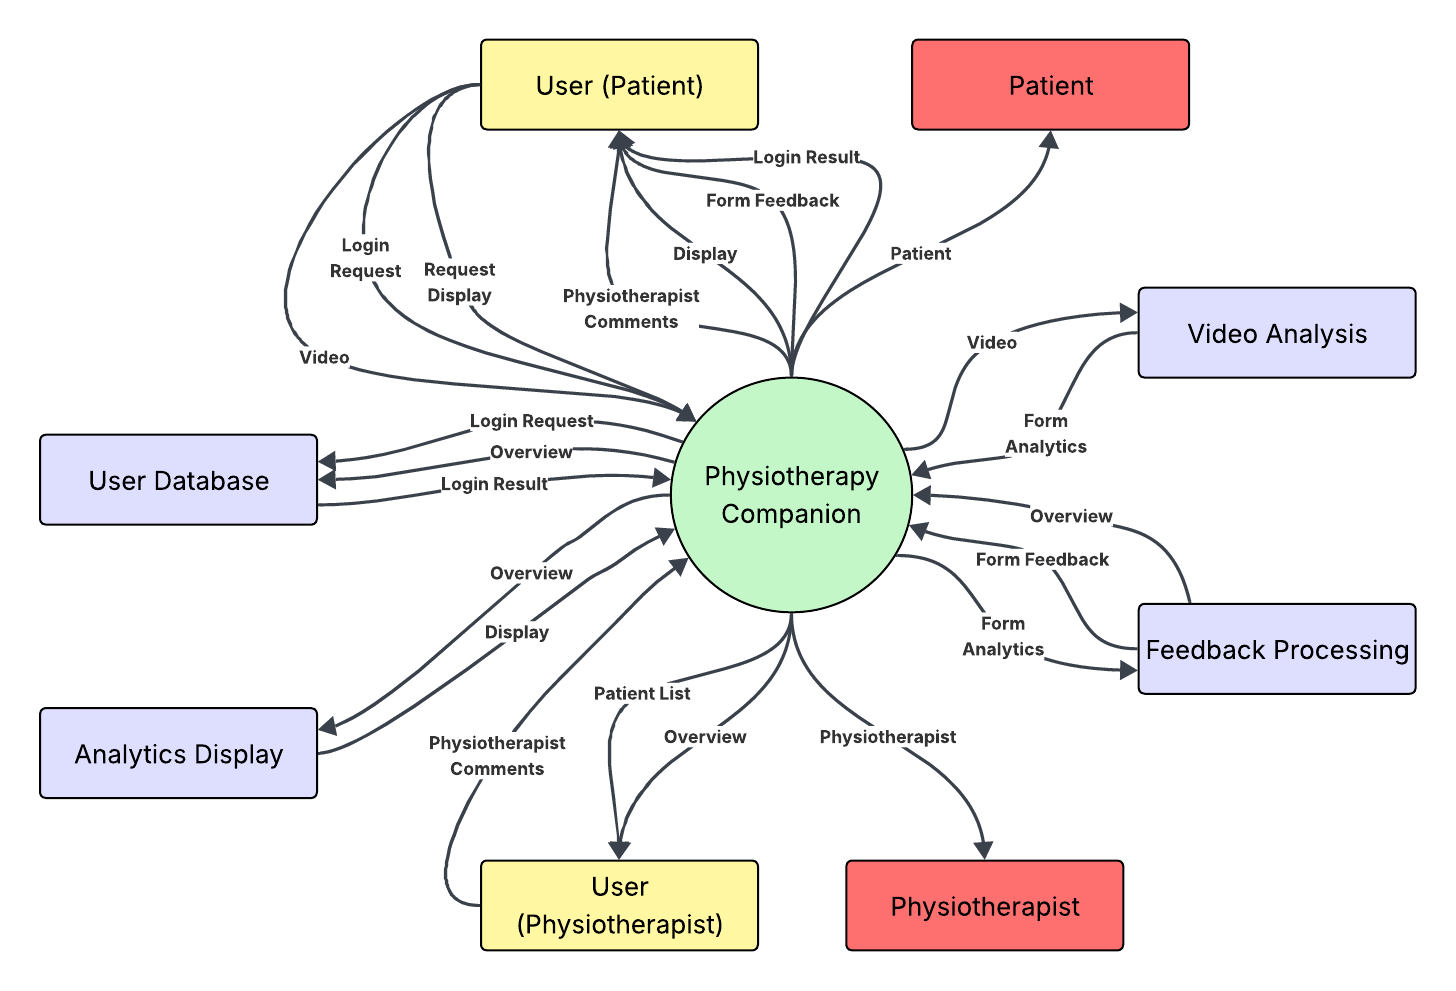
\includegraphics[width=\linewidth]{Context_Diagram.png}
  \caption{Work Context Diagram}
\end{figure}

\subsection{Work Partitioning}
\begin{table}[H]
\centering
\begin{tabular}{|m{3cm}|m{3cm}|m{8cm}|}
  \hline
  \textbf{Event} & \textbf{System Action} & \textbf{Description} \\ \hline
  User Requests Login & Login Request (in) & Compare user’s entered data with user database. \\ \hline
  Login Result Return & Login Result (out) & Return result, login or fail, to user based on data comparison. \\ \hline
  User Requests Display & Display Request (in) & Generate display with data from the user database. \\ \hline
  Display Return & Display Return (out) & Send the generated display to the user's GUI. \\ \hline
  User Submits Video & Form Feedback Request (in) & The user submits a video-feed for form analysis. \\ \hline
  Form Feedback Return & Form Feedback Return (out) & The system analyzes the form in the user’s video feed. The system generates form feedback and an overview from the analyzed information. The system generates a display with the newly added overview. The system sends the form feedback and the new display to the user. \\ \hline  
\end{tabular}
\caption{Work Partitioning}
\end{table}

\subsection{Specifying a Business Use Case (BUC)}
A user (patient) is prescribed exercises by a physiotherapist and uses the app to ensure they are doing the exercises correctly. This use case assumes the user is already logged in, and thus skips the login steps.

\begin{figure}[H]
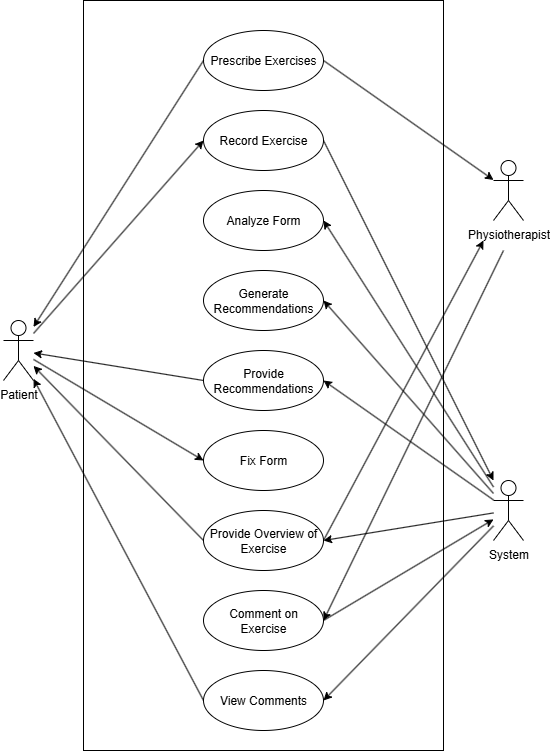
\includegraphics[width=\linewidth]{BUC.png}
\caption{Business Use Case Diagram}
\end{figure}

\section{Business Data Model and Data Dictionary}
\subsection{Business Data Model}
N/A 
This is not yet concrete, and will be fleshed out more at the implementation stage. Currently, the data flow should look very similar to that seen in the Work Context Diagram.

\subsection{Data Dictionary}
N/A
For the same reasons above, the data structures and specific metadata required for this section doesn’t yet exist within the project, and so cannot be entered here.

\section{The Scope of the Product}
\subsection{Product Boundary}
Refer to the Work Context Diagram for the boundaries of the system’s operations.
\subsection{Product Use Case Table}
\begin{figure}[H]
  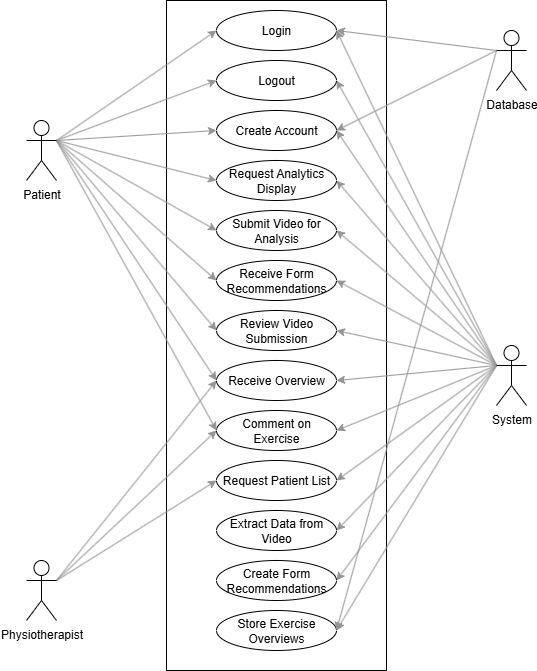
\includegraphics[width=13cm]{PUC.png}
  \caption{Product Use Case Table}
\end{figure}
\subsection{Individual Product Use Cases (PUC's)}
Where not specified, user is assumed to be user (patient).\\ \\
PUC1: Login\\
Event: User enters username and password and requests login.\\
Preconditions: User is not logged in.\\
Actors: User, System, Database\\
Normal Flow: User enters a valid username and password confirmed within the database and successfully accesses their pre-existing account.\\
Alternative Flow: User enters an invalid username and password which don’t verify in the database and the user is returned an error for invalid login information.\\ \\
PUC2: Logout\\
Event: User requests to logout of their account.\\
Preconditions: User is logged in.\\
Actors: User, System\\
Normal Flow: User requests to log out of their account. The system moves the user to the login page.\\
Alternative Flow: N/A\\ \\
PUC3: Create Account\\
Event: User requests to create an account.\\
Precondition: User is not logged in.\\
Actors: User, System, Database\\
Normal Flow: User enters an email, username, and password combination not already contained within the database. Email and username must be unique. The system creates an account for the user, stores the account information in the user database, and logs them into their account.\\
Alternative Flow: User enters an email or username that already exists within the user database, or a password which does not meet minimum requirements. The system returns an error and prompts the user to re-enter incorrect fields.\\ \\
PUC4: Request Analytics Display\\
Event: User refreshes analytics display (home page), user logs into their account, user returns to home page after an exercise.
Precondition: User is logged in and on the home page.\\
Actors: User, System\\
Normal Flow: After any of the events, the system uses all the stored user exercise overviews to refresh the analytics display.\\
Alternative Flow: If there are no stored exercise overviews for the user, the system prompts them to complete an exercise.\\ \\
PUC5: Submit Video for Analysis\\
Event: User submits a video-feed for form analysis.\\
Precondition: User is logged in and on the video submission screen.\\
Actors: User, System\\
Normal Flow: User submits a video-feed to the system for form analysis. The system accepts the video and recognizes the patient (user) within the video.\\
Alternative Flow: The system doesn’t recognize a patient within the video and prompts the user to fix any issues with their video-feed.\\ \\
PUC6: Receive Form Recommendations\\
Event: User is logged in and has submitted a video-feed for form analysis.\\
Precondition: User is logged in and the system has recognized them within the video-feed.\\
Actors: User, System\\
Normal Flow: System returns form recommendations based on data pulled from the video-feed and formulates the data into readable language recommendations which are displayed to the user.\\
Alternative Flow: System fails to draw analytical information from the video-feed and fails to create form recommendations for the patient (user).\\ \\
PUC7: Review Video Submission\\
Event: User has ended the video-feed upload.\\
Precondition: User is logged in, has submitted a video-feed for analysis, and has successfully received form recommendations.\\
Actors: User, System\\
Normal Flow: User can rewatch their video-feed submission with form recommendations in real-time before finally exiting the video submission screen.\\
Alternative Flow: User can cancel or request to redo their video-feed submission, taking them back to PUC5.\\ \\
PUC8: Receive Overview\\
Event: User has submitted and exited a video-feed submission.\\
Precondition: User has successfully submitted a video-feed submission, received recommendations, and exited the submission screen.\\
Actors: User (Patient), User (Physiotherapist), System\\
Normal Flow: System generates an overview of the exercise just submitted by the user and provides in natural language an overview to the user.\\
Alternative Flow: If the user didn’t submit their video-feed but exited and cancelled instead, no overview is created.\\ \\
PUC9: Comment on Exercise\\
Event: User creates a comment on an exercise.\\
Precondition: User (Patient) must be logged in and have completed one exercise, or, user (Physiotherapist) must be logged in and have at least one patient that has completed one exercise.\\
Actors: User (Patient), User (Physiotherapist), System\\
Normal Flow: User requests to create a comment on an exercise overview. User enters their own information into a text field and submits the comment. This comment is now visible to all users with access to that exercise overview.\\
Alternative Flow: User cancels their comment creation, and no comment is saved alongside the exercise overview.\\ \\
PUC10: Request Patient List\\
Event: User (Physiotherapist) requests or refreshes the patient list on their homepage.\\
Precondition: User (Physiotherapist) is logged in.\\
Actors: User (Physiotherapist), System\\
Normal Flow: System returns the list of all patients tied to the respective user (Physiotherapist) account, with access to their exercise overviews.\\
Alternative Flow: If the user (Physiotherapist) has no patients connected to their account, the system prompts them to add at least one patient.\\ \\
PUC11: Extract Data from Video\\
Event: System receives a video-feed from a user.\\
Precondition: User is recognizable in the video-feed.\\
Actors: System\\
Normal Flow: The system uses a CV library to extract necessary data relevant to the user’s form, storing the information locally for generating form recommendations, analytics displays, and overviews.\\ \\
PUC12: Create Form Recommendation\\
Event: System has extracted necessary form data from a video-feed.\\
Precondition: The video-feed was successfully analyzed by the CV library and received the necessary information.\\
Actors: System\\
Normal Flow: The system takes the form data and generates a naturally worded recommendation for the user’s form.\\ \\
PUC13: Store Exercise Overview\\
Event: Exercise overview has been created, comment has been submitted.\\
Precondition: Exercise overview or comment was successfully created, not cancelled.\\
Actors: System, Database\\
Normal Flow: The exercise overview is stored in the user database tied to the user’s account.\\

\subsection{System State Diagram}
\begin{figure}[H]
  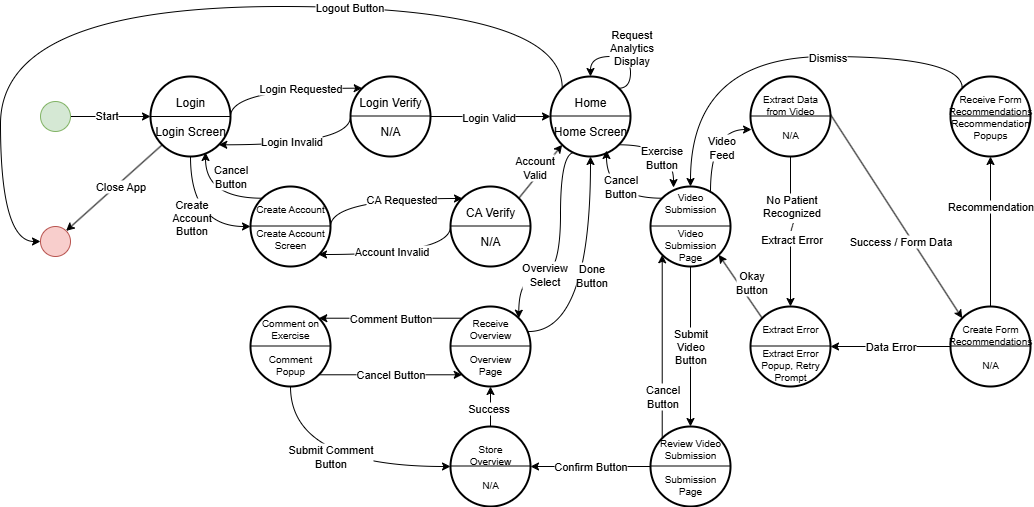
\includegraphics[width=\linewidth]{FSM.png}
  \caption{System State Diagram (State Machine)}
\end{figure}

\section{Functional Requirements}

\begin{reqlist}
	
	\item[FR 1.] The system shall require returning users to log in with unique credentials before accessing any exercise or dashboard features.
	\rationale{Authentication ensures that patient data remains private and that exercise programs are accessed only by the intended individual, maintaining accountability for treatment compliance.}
	\fitcrit{The system prevents access to any exercise or dashboard features without successful authentication. Unauthorized access attempts are rejected 100\% of the time.}
	
	\item[FR 1.1] The system shall require a new user to create an account with unique credentials as the appropriate user role (Physiotherapist or Patient) and complete all the required fields to verify account creation.
	\rationale{Role-based account creation ensures that users are granted appropriate access permissions from the outset, preventing unauthorized access to certain features. Requiring all fields to be completed ensures that essential information needed for system functionality and regulatory compliance is collected during registration, reducing incomplete profiles and data quality issues.}
	\fitcrit{The system rejects account creation attempts with missing required fields or duplicate credentials. All new accounts are successfully assigned to the correct user role (PT or Patient) with appropriate permissions activated upon creation.}
	
	\item[FR 1.2] The system shall require a physiotherapist user to provide a PT license from their provincial regulatory body, a government ID, registration number/client ID, and location and ID of their practicing clinic in order to join the clinic’s organization on the app.
	\rationale{Verifying PT credentials through provincial regulatory body information ensures that only licensed, qualified healthcare professionals can provide clinical services through the system. This protects patient safety, maintains professional standards, ensures regulatory compliance, and reduces liability by preventing unauthorized individuals from accessing patient data or prescribing treatment. Linking PTs to specific clinics enables proper organizational management and accountability.}
	\fitcrit{The system requires all four credential fields (PT license, government ID, registration number, clinic location/ID) to be completed before allowing PT access. Incomplete credential submissions are rejected, and PTs without verified credentials cannot access patient data or clinical features.}
	
	\item[FR 1.3] The system shall require a user to enter a unique code provided by their Physiotherapist in order to join the correct organization and interact with their PT through the system.
	\rationale{A unique access code creates a secure connection between patients and their specific physiotherapist within the correct clinic organization. This prevents patients from accidentally joining the wrong organization or connecting with an incorrect PT, ensures proper care continuity, and maintains organizational boundaries. The code-based approach provides a simple yet effective authentication method that doesn't require complex user verification processes while maintaining security.}
	\fitcrit{Patients cannot join an organization without entering a valid unique code. Invalid or expired codes are rejected 100\% of the time. Each code successfully links the patient to exactly one PT and one organization.}
	
	\item[FR 2.] The system shall allow a physiotherapist user (PT) to create, initialize, and manage patient accounts, including assigning patients a code to join their own organization.
	\rationale{Physiotherapists are licensed medical professionals responsible for patient care and must maintain control over who accesses the system to ensure proper supervision and treatment oversight.}
	\fitcrit{PTs can successfully create patient accounts, generate unique access codes, and perform account management functions (edit, disable, reset) for all patients under their care. All PT-initiated account actions are logged and executed without errors.}
	
	\item[FR 3.] The system shall restrict patients from joining a clinic’s organization independently; all accounts must be authorized by a physiotherapist.
	\rationale{This prevents unauthorized access to medical treatment tools and ensures that only patients under active care can use the system, maintaining professional oversight and reducing liability.}
	\fitcrit{Patient attempts to join an organization without PT authorization (valid unique code) are rejected 100\% of the time. All active patient accounts can be traced back to a PT-initiated authorization.}
	
	\item[FR 4.] The system shall allow physiotherapists to reset or disable patient accounts if misuse or inactivity is detected.
	\rationale{Account management capabilities enable PTs to respond to security concerns, terminate care when treatment is complete, and maintain system integrity.}
	\fitcrit{PTs can successfully reset passwords and disable patient accounts within 60 seconds. Disabled accounts immediately lose access to all system features. All reset and disable actions are logged with timestamps and PT identifiers.}
	
	\item[FR 5.] The system shall provide patients with guided exercise instructions for the knee joint (first iteration).
	\rationale{Focusing on knee joint exercises for the initial release allows the development team to create a robust, well-tested foundation before expanding to other joint types, reducing complexity and time-to-market.}
	\fitcrit{The system includes a complete library of at least 10 common knee rehabilitation exercises with step-by-step instructions, demonstration videos or images, and proper form guidelines. Instructions are accessible to all authorized patients.}
	
	\item[FR 6.] The system shall allow physiotherapists to assign, customize, and update prescribed exercises (e.g., number of sets, reps, rest time).
	\rationale{Each patient has unique needs and progress rates. Customization enables PTs to tailor treatment plans to individual capabilities, injuries, and recovery stages for optimal therapeutic outcomes.}
	\fitcrit{PTs can modify at least three parameters (sets, reps, rest time) for any assigned exercise. Changes are saved and immediately reflected in the patient's exercise program. The system tracks all modifications with timestamps.}
	
	\item[FR 7.] The system shall allow patients to record their exercise attempts through video capture.
	\rationale{Video recording provides objective documentation of patient performance, enabling both real-time computer vision analysis and later review by physiotherapists for comprehensive assessment.}
	\fitcrit{Patients can successfully initiate and complete video recording of exercise attempts using their device camera. Videos are captured at minimum 720p resolution and 30fps, and are stored for PT review.}
	
	\item[FR 8.] The system shall support retry attempts if the patient's form does not meet alignment requirements.
	\rationale{Allowing retries encourages patients to achieve correct form, which is essential for injury prevention, therapeutic effectiveness, and building proper movement patterns.}
	\fitcrit{When form deviations are detected, the system prompts the patient to retry and allows unlimited retry attempts until correct form is achieved or the patient chooses to stop. Each retry attempt is recorded separately.}
	
	\item[FR 9.] The system shall prompt the user to provide feedback on the level of difficulty of the exercise, effectiveness, and the patient's satisfaction with the given exercise.
	\rationale{Patient feedback provides valuable qualitative data that complements quantitative performance metrics, helping PTs adjust treatment plans based on patient experience and perceived progress.}
	\fitcrit{After each exercise session, the system prompts patients to rate difficulty, effectiveness, and satisfaction on a defined scale (e.g., 1--5 or 1--10). Feedback is captured and stored with the exercise session data. The system prevents session completion until feedback is provided or explicitly skipped.}
	
	\item[FR 10.] The system shall provide patients with an overview of completed and pending exercises, including suggested progressions.
	\rationale{Progress visibility motivates patients, helps them understand their treatment trajectory, and promotes adherence by showing accomplishments and next steps.}
	\fitcrit{The patient dashboard displays a complete list of assigned exercises showing completion status, completion dates, and suggested next exercises. The overview updates in real-time as exercises are completed.}
	
	\item[FR 11.] The system shall capture exercise metadata such as frequency, duration, number of repetitions, rest periods, and pain scores.
	\rationale{Comprehensive metadata enables PTs to track adherence, identify patterns, assess progress objectively, and make data-driven decisions about treatment modifications.}
	\fitcrit{For each exercise session, the system automatically captures and stores at least five metadata fields (frequency, duration, repetitions, rest periods, pain scores). All metadata is timestamped and associated with the correct patient and exercise.}
	
	\item[FR 12.] The system shall analyze captured video streams using computer vision to compute biomechanical features (e.g., joint angle, range of motion, time-under-tension).
	\rationale{Automated biomechanical analysis provides objective, quantitative measurements that would be difficult or impossible to obtain manually, enabling precise assessment of exercise execution quality.}
	\fitcrit{The system successfully computes at least three biomechanical measurements (joint angle, range of motion) from video with $\pm5^\circ$ accuracy for angles and $\pm10\%$ accuracy for time measurements when compared to manual expert assessment.}
	
	\item[FR 13.] The system shall compare patient performance against reference exercise models to verify correctness of form.
	\rationale{Comparing against validated reference models ensures that the system's feedback is based on established therapeutic standards and best practices for each exercise type.}
	\fitcrit{The system compares patient performance metrics against stored reference models and generates a form correctness score or pass/fail determination for each exercise attempt. Comparison results are provided to both patient and PT.}
	
	\item[FR 14.] The system shall provide corrective feedback highlighting deviations (e.g., insufficient bend, poor alignment, incorrect tempo).
	\rationale{Specific, actionable feedback helps patients understand and correct mistakes in real-time, improving exercise quality and reducing the risk of injury or ineffective treatment.}
	\fitcrit{When form deviations are detected, the system provides specific feedback identifying the type of deviation (e.g., ``insufficient knee bend,'' ``poor hip alignment'') within 1 second of detection. Feedback includes both visual and audible cues.}
	
	\item[FR 15.] The system shall allow patients to review recorded exercise attempts before submission.
	\rationale{Self-review empowers patients to evaluate their own performance, promotes self-awareness of movement quality, and allows them to decide whether to retry before submitting to their PT.}
	\fitcrit{Patients can replay their recorded exercise video immediately after completion and before submission. The review interface includes playback controls (play, pause, rewind) and displays form analysis results alongside the video.}
	
	\item[FR 16.] The system shall prompt patients to retry until correct alignment is achieved.
	\rationale{Persistent prompting ensures that patients develop correct movement patterns and don't reinforce poor form, which is critical for therapeutic success and injury prevention.}
	\fitcrit{After each failed attempt, the system displays a retry prompt with specific guidance on what to correct. The system continues prompting until the patient achieves passing form or manually chooses to end the session.}
	
	\item[FR 17.] The system shall generate session-based and daily progress reports for physiotherapists.
	\rationale{Regular automated reports enable PTs to efficiently monitor multiple patients, identify trends, and intervene quickly when issues arise without manually reviewing all exercise attempts.}
	\fitcrit{The system automatically generates reports after each session and compiles daily summaries by end of day. Reports include completion rates, form scores, pain levels, and patient feedback. PTs can access reports within 5 seconds of generation.}
	
	\item[FR 18.] The system shall provide physiotherapists with dashboards listing patients, their progress, and flagged cases.
	\rationale{Centralized dashboards allow PTs to prioritize their attention, quickly identify patients who need intervention, and manage their caseload efficiently.}
	\fitcrit{The PT dashboard displays all patients in the PT's caseload with summary statistics (adherence rate, average form score, days since last session). Cases requiring attention are visually flagged and sortable. Dashboard loads within 2 seconds.}
	
	\item[FR 19.] The system shall allow physiotherapists to leave feedback on patient submissions.
	\rationale{Direct PT feedback provides personalized guidance, reinforces correct behavior, addresses specific concerns, and maintains the therapeutic relationship in a remote care setting.}
	\fitcrit{PTs can view any patient submission and add text or voice feedback. Feedback is immediately visible to the patient and timestamped. The system supports feedback of at least 500 characters or 2 minutes of voice recording.}
	
	\item[FR 20.] The system shall alert physiotherapists if a patient repeatedly fails to complete exercises correctly.
	\rationale{Automatic alerts ensure that PTs are notified of potential issues requiring intervention, preventing patients from continuing ineffective or potentially harmful exercise patterns.}
	\fitcrit{The system generates an alert to the PT when a patient fails the same exercise 3 consecutive times or fails to achieve passing form in 5 attempts across any exercises within a 7-day period. Alerts appear prominently on the PT dashboard.}
	
	\item[FR 21.] The system shall securely store all patient data, including personal details, medical history, and exercise logs.
	\rationale{Comprehensive data storage is necessary for continuity of care, legal documentation, treatment planning, and compliance with medical record-keeping requirements.}
	\fitcrit{All patient data (personal information, medical history, exercise logs, videos) is stored in the database with no data loss. Data retrieval succeeds 99.9\% of the time. Storage implements encryption at rest and backup procedures.}
	
	\item[FR 22.] The system shall allow physiotherapists to update and manage patient records.
	\rationale{PTs need the ability to maintain accurate, up-to-date records as patient conditions change, treatments progress, and new information becomes available.}
	\fitcrit{PTs can successfully edit patient information fields, add medical history notes, and update treatment plans. All changes are saved with timestamps and version history. Updates are reflected immediately in the patient record.}
	
	\item[FR 23.] The system shall restrict patients to accessing only their own data.
	\rationale{Data access restrictions protect patient privacy, comply with healthcare privacy regulations, and prevent unauthorized disclosure of sensitive medical information.}
	\fitcrit{Patients can only view and interact with data associated with their own account. Attempts to access other patients' data through URL manipulation or other means are blocked 100\% of the time.}
	
	\item[FR 24.] The system shall store only the biomechanical metrics and performance data extracted from video analysis; raw video recordings shall not be retained on the server.
	\rationale{Storing only derived metrics rather than raw video reduces privacy risk and storage burden while still providing PTs with all data needed for clinical decision-making. This approach limits exposure of sensitive patient imagery and simplifies compliance with PIPEDA and provincial health privacy legislation.}
	\fitcrit{Raw video recordings are processed on-device and discarded after metric extraction is complete. No video files are transmitted to or persisted on the server. The system stores only computed metrics (e.g., joint angles, rep counts, pain scores) associated with each session. Compliance is verified by confirming no video data exists in the server database following session completion.}
	
	\item[FR 25.] The system shall ensure video and performance data are available for PT review and decision-making.
	\rationale{Timely access to performance data enables PTs to make informed clinical decisions, adjust treatment plans appropriately, and provide evidence-based care.}
	\fitcrit{PTs can access patient videos and performance data within 5 seconds of request. Data availability is maintained at 99\% uptime. Videos and data are synchronized and viewable within 1 minute of patient submission.}
	
	\item[FR 26.] The system shall support retry attempts if the patient's form has insufficient data.
	\rationale{Insufficient data (due to occlusion, poor camera angle, or movement out of frame) prevents accurate form assessment and makes corrective feedback impossible. Allowing retries when data is incomplete gives patients another opportunity to capture usable video rather than submitting unusable attempts to their PT. This improves data quality, ensures that PTs receive meaningful performance information, and prevents patients from being incorrectly flagged for poor form when the issue was actually technical rather than performance-based.}
	\fitcrit{When video analysis detects insufficient data (e.g., patient out of frame, excessive occlusion), the system alerts the patient with a specific reason and prompts for retry. The system allows unlimited retries until sufficient data quality is achieved.}
	
	\item[FR 27.] The system shall allow for physiotherapists to input daily/weekly limitations on the metrics measured by the application.
	\rationale{Patient recovery is progressive, and safe exercise parameters change over time based on healing, pain levels, and functional improvement. Allowing PTs to set temporal limitations (e.g., ``no more than 3 sets per day this week'' or ``maintain knee flexion under 90 degrees for the next 5 days'') enables precise, time-bound treatment modifications that adapt to patient progress. This supports clinical best practices of gradual progression, helps prevent overexertion during vulnerable recovery phases, and gives PTs fine-grained control over treatment intensity.}
	\fitcrit{PTs can set time-bound parameter limits (daily/weekly) for at least three metrics (sets, reps, range of motion thresholds). The system enforces these limits automatically, preventing patients from exceeding them. Limits can be modified or removed at any time by the PT.}
	
\end{reqlist}

\section{Look and Feel Requirements}

\subsection{Appearance Requirements}
\begin{reqlist}
	\item[LFR-AP 1.] The system shall maintain consistent navigation and design across all interfaces.
	\rationale{Consistency reduces cognitive load, minimizes learning time, and prevents user confusion when navigating between different features of the application.}
	\fitcrit{All interfaces use the same navigation structure, color scheme, typography, and button styles. User testing confirms that 90\% of users can navigate between features without assistance after a 5-minute introduction.}
\end{reqlist}

\subsection{Style Requirements}
\begin{reqlist}
	\item[LFR-ST 1.] The system shall provide a user-friendly interface with clear instructions and visual cues.
	\rationale{Many patients and some PTs may have limited technical expertise. A clear, intuitive interface ensures that the technology doesn't become a barrier to receiving or providing care.}
	\fitcrit{User testing with participants of varying technical skill levels shows that 80\% can complete common tasks (start exercise, view progress, leave feedback) without external help. All critical actions have visible instructions and visual indicators.}
\end{reqlist}

\section{Usability and Humanity Requirements}

\subsection{Ease of Use Requirements}
\begin{reqlist}
	\item[UHR-EOU 1.] The system shall be accessible to users with limited technical skills.
	\rationale{The patient population includes individuals of all ages and technical abilities. The system must accommodate users who may not be comfortable with complex technology to ensure broad accessibility.}
	\fitcrit{User testing with participants aged 18--75 with varying technical proficiency shows that 80\% can complete basic tasks (login, start exercise, submit video) within 10 minutes without training.}
	
	\item[UHR-EOU 2.] The system shall provide patients with real-time corrective feedback (audible/visual cues) while performing exercises.
	\rationale{Immediate feedback during exercise execution allows patients to correct their form in real-time, maximizing therapeutic benefit and reducing the risk of injury from improper technique.}
	\fitcrit{Corrective feedback (both audible prompts and visual indicators) is delivered within 1 second of detecting form deviation. Feedback is synchronized with patient movement throughout the exercise session.}
	
	\item[UHR-EOU 3.] The system shall prompt the user at the start of video streaming if there are obstructions or low-light levels and give the user a chance to change their environment prior to analysis.
	\rationale{Proactive environmental checks prevent wasted exercise sessions due to poor video quality. By alerting users to obstructions or lighting issues before they begin, the system helps ensure that computer vision analysis will be accurate and that corrective feedback will be meaningful. This improves user satisfaction by preventing frustration from having to repeat exercises due to technical issues rather than form problems, and it ensures the quality of data collected for PT review.}
	\fitcrit{The system detects low-light conditions and obstructions before exercise begins. Detection occurs within 3 seconds of camera activation. Users receive clear prompts with suggestions for improvement.}
	
	\item[UHR-EOU 4.] The system shall prompt the user if the application does not have access to the camera or if there is an alternative program that is using the camera.
	\rationale{Camera access is fundamental to the system's functionality. Clear prompts help users quickly identify and resolve permission issues or conflicts with other applications, preventing confusion and technical support calls. Many users may not understand why video capture isn't working without explicit notification. This guidance enables users to troubleshoot independently, reducing barriers to system use and improving the overall user experience.}
	\fitcrit{When camera access is denied or the camera is in use by another application, the system displays a specific error message within 2 seconds explaining the issue and providing resolution steps. The prompt includes platform-specific instructions for granting camera permissions.}
	
	\item[UHR-EOU 5.] The system shall provide a guideline overlay when setting up the smart device so they are in-frame of the view and correct orientation.
	\rationale{Proper camera positioning and device orientation are critical for accurate computer vision analysis of exercise form. A visual guideline overlay (such as body outline or positioning markers) helps users set up their device correctly without trial and error. This reduces setup frustration, ensures consistent data quality across sessions, improves the accuracy of biomechanical analysis, and helps users understand the spatial requirements for effective system operation.}
	\fitcrit{The system displays a visual overlay (body outline or frame markers) during setup. The overlay provides real-time feedback when the user is correctly positioned (green indicator) or needs adjustment (red/yellow indicator with directional guidance).}
	
	\item[UHR-EOU 6.] The system shall provide an option to view the motion on an internal page on the application to help guide the motion during analysis.
	\rationale{Real-time visual feedback showing patients their own movement as the system analyzes it helps them understand what the computer vision system ``sees'' and make immediate adjustments. This self-awareness tool bridges the gap between feeling correct and actually performing correctly, particularly useful for proprioceptive deficits common after injury. Seeing themselves on screen helps patients correlate system feedback with their actual movement, improving form correction accuracy and building better movement patterns through visual-kinesthetic integration.}
	\fitcrit{Patients can activate a live video feed view showing themselves during exercise execution. The view is available as an optional toggle on the exercise interface and updates in real-time throughout the session.}
\end{reqlist}

\subsection{Personalization and Internationalization Requirements}
N/A

\subsection{Learning Requirements}
\begin{reqlist}
	\item[UHR-LRN 1.] The system shall provide clear instructions for exercise execution and system navigation.
	\rationale{Clear instructions reduce the learning curve, improve user confidence, ensure exercises are performed correctly, and minimize the need for external support.}
	\fitcrit{Each exercise includes written instructions (maximum 8th-grade reading level) and visual demonstrations. Navigation instructions are available on first use.}
\end{reqlist}

\subsection{Understandability and Politeness Requirements}
\begin{reqlist}
	\item[UHR-UPL 1.] The system shall provide corrective feedback in a clear and constructive manner.
	\rationale{Constructive, respectful feedback maintains patient motivation and engagement. Harsh or confusing feedback could discourage patients from continuing their treatment program.}
	\fitcrit{All feedback messages use positive, instructive language (e.g., ``Try bending your knee a bit more'' rather than ``Wrong'').}
\end{reqlist}

\subsection{Accessibility Requirements}
\begin{reqlist}
	\item[UHR-AR 1.] The system shall provide both visual and audible cues.
	\rationale{The system providing different methods to indicate whether a patient is correctly performing exercises or not ensures accessibility to users who benefit in understanding the functionalities and instructions given by the application.}
	\fitcrit{All critical feedback and instructions are available in both visual (on-screen text/graphics) and audible (spoken) formats.}
\end{reqlist}

\section{Performance Requirements}

\subsection{Speed and Latency Requirements}
\begin{reqlist}
	\item[PR-SL 1.] The system shall load the exercise interface within 2 seconds under normal network conditions.
	\rationale{Fast loading times prevent user frustration and abandonment. Patients are more likely to complete exercises when the system responds quickly, maintaining treatment adherence.}
	\fitcrit{The exercise interface loads completely (all elements interactive) within 2 seconds on a standard connection.}
	
	\item[PR-SL 2.] The system shall process video feedback and deliver corrective cues within 1 second of detected motion.
	\rationale{Real-time feedback requires minimal latency to be effective. Delayed feedback may occur after the patient has already moved to the next repetition, making corrections impossible to implement immediately.}
	\fitcrit{From the moment a form deviation is detected in the video stream, corrective feedback (visual and audible) is delivered within 1 second in 95\% of cases. Latency is measured from deviation occurrence to feedback display.}
	
	\item[PR-SL 3.] The system shall complete the upload of a typical exercise video file to the server within 60 seconds under normal network conditions.
	\rationale{Timely upload ensures patients receive session confirmation and that PTs have access to performance data without excessive delay. Long upload times reduce engagement and disrupt the post-exercise workflow.}
	\fitcrit{A video file of 50~MB or less uploads successfully and receives a server acknowledgment within 60 seconds on a connection with a minimum 10~Mbps upload speed. A success notification is displayed to the user upon confirmed upload completion.}
	\end{reqlist}

\subsection{Safety-Critical Requirements}
\begin{reqlist}
	\item[PR-SCR 1.] The system shall not allow patients to proceed with exercises if critical form violations are detected that could result in injury.
	\rationale{Preventing exercise execution when dangerous form is detected protects patients from potential injury, particularly when performing unsupervised exercises at home. This overrides the general principle of allowing retries to prioritize immediate safety.}
	\fitcrit{When critical form violations (defined as deviations $>30^\circ$ from safe range or joint stress indicators) are detected, the system immediately halts the exercise with a warning message. The system prevents continuation until the violation is corrected.}
\end{reqlist}

\subsection{Precision or Accuracy Requirements}
\begin{reqlist}
	\item[PR-PAR 1.] The system shall accurately compute biomechanical features (e.g., joint angle, range of motion) with sufficient precision to detect form deviations.
	\rationale{Accurate measurements are essential for providing valid feedback and tracking progress. Inaccurate measurements could lead to inappropriate corrections or missed therapeutic opportunities.}
	\fitcrit{Joint angle measurements are accurate within $\pm5^\circ$ compared to manual goniometer measurements by a trained physiotherapist. Range of motion calculations are within $\pm10\%$ of expert assessment in 90\% of test cases.}
	
	\item[PR-PAR 2.] The system shall compare patient performance against reference exercise models with sufficient accuracy to verify correctness of form.
	\rationale{Form verification accuracy directly impacts therapeutic effectiveness and patient safety. False positives or negatives could reinforce poor form or discourage correct performance.}
	\fitcrit{Form verification achieves minimum 85\% accuracy (correctly identifies both correct and incorrect form) when compared to expert PT assessment. False positive rate is below 10\%, and false negative rate is below 15\%.}
\end{reqlist}

\subsection{Robustness or Fault-Tolerance Requirements}
\begin{reqlist}
	\item[PR-RFT 1.] The system shall recover from unexpected failures within 5 minutes.
	\rationale{Quick recovery minimizes disruption to patient exercise sessions and prevents data loss. Extended downtime could cause patients to miss treatment windows or lose confidence in the system.}
	\fitcrit{System recovery from crashes or errors completes within 5 minutes, with all patient data preserved. Recovery success rate is 95\%. Users can resume their session without re-entering data or repeating completed exercises.}
	
	\item[PR-RFT 2.] The system shall queue and re-attempt submissions if internet connectivity fails during video upload.
	\rationale{Home internet connections may be unreliable. Automatic retry mechanisms ensure that patient work is not lost and PTs receive all performance data despite temporary connectivity issues.}
	\fitcrit{Failed uploads are automatically queued locally and retry every 30 seconds until successful.}
	
	\item[PR-RFT 3.] The system shall maintain an uptime of at least 99\% during operational hours.
	\rationale{High availability ensures that patients can access their treatment programs when scheduled. Frequent downtime could disrupt treatment adherence and patient outcomes.}
	
	\item[PR-RFT 4.] The system shall monitor the smart device's battery life and prompt the user if it falls below a certain threshold to charge the device.
	\rationale{Exercise sessions interrupted by device power loss result in lost data, incomplete PT records, and user frustration. Proactive battery monitoring allows users to charge their device or complete a shorter session before power runs out. This is particularly important for video recording and analysis, which can drain the battery quickly. Preventing mid-session failures improves data completeness, user experience, and treatment adherence by ensuring sessions can be completed successfully.}
\end{reqlist}

\subsection{Capacity Requirements}
\begin{reqlist}
	\item[PR-CR 1.] The system shall support at least 100 concurrent users without degradation in performance.
	\rationale{High availability ensures that patients can access their treatment programs when scheduled. Frequent downtime could disrupt treatment adherence and patient outcomes.}
	\fitcrit{Load testing confirms the system supports 100 simultaneous active sessions with response times remaining within specified limits (2-second interface load, 1-second feedback delivery). No crashes or errors occur under maximum load conditions.}
\end{reqlist}

\subsection{Scalability or Extensibility Requirements}
\begin{reqlist}
	\item[PR-SER 1.] The system architecture shall support future expansion to additional joint types beyond the knee.
	\rationale{Starting with knee exercises but planning for expansion ensures the system can grow to serve broader treatment needs without requiring complete architectural redesign.}
	\fitcrit{System architecture uses modular, joint-agnostic design patterns. Adding a new joint type (e.g., shoulder, ankle) requires only new exercise definitions and reference models, not core system changes.}
\end{reqlist}

\subsection{Longevity Requirements}
\noindent N/A \\
\textit{Reason:} Longevity requirements have been addressed in the previous iteration and are now covered under requirements 12.7.1 and 12.7.2, which specify a minimum 5-year operational lifespan and the use of widely-supported, non-proprietary technologies. No additional longevity requirements are necessary at this stage of the project.

\section{Operational and Environmental Requirements}

\subsection{Expected Physical Environment}
\begin{reqlist}
	\item[OER-EP 1.] The system shall function in typical home and clinical environments where patients perform physiotherapy exercises.
	\rationale{Patients will use the system in diverse settings with varying lighting, space constraints, and background conditions. The system must be robust enough to function reliably in non-laboratory environments.}
	\fitcrit{Computer vision analysis functions accurately in lighting conditions from 200--1000 lux, with backgrounds containing typical home elements (furniture, walls, patterns). Testing in 5 diverse home environments shows successful exercise capture and analysis in 90\% of cases.}
\end{reqlist}

\subsection{Wider Environment Requirements}
\begin{reqlist}
	\item[OER-WE 1.] The system shall be compatible with major operating systems (Windows, iOS, Android).
	\rationale{Patients and PTs use diverse devices and operating systems. Cross-platform compatibility ensures maximum accessibility and prevents the system from excluding users based on their device choices.}
	\fitcrit{The system installs and runs without errors on Windows 10+, iOS 14+, and Android 10+. All core features function identically across platforms. Cross-platform testing shows 95\% feature parity.}
	
	\item[OER-WE 2.] The system shall adapt to both mobile and desktop screen resolutions.
	\rationale{Users may prefer different devices based on context (e.g., mobile for exercises, desktop for PT review). Responsive design ensures usability across all common screen sizes.}
	\fitcrit{The interface adapts to screen sizes from 5-inch mobile devices to 27-inch desktop monitors. All interface elements remain accessible and readable. No horizontal scrolling is required. Testing on 10 different screen sizes shows full functionality on all devices.}
\end{reqlist}

\subsection{Requirements for Interfacing with Adjacent Systems}
\noindent N/A \\
\textit{Reason:} Interface requirements have been addressed in the previous iteration and are now covered under requirements 13.3.1 and 13.3.2, which specify API integration capabilities for EMR systems and standardized data export formats. The first iteration of the system focuses on core functionality as a standalone application.

\subsection{Productization Requirements}
\begin{reqlist}
	\item[OER-PR 1.] The system shall include comprehensive user documentation for both patients and physiotherapists, including setup guides, troubleshooting instructions, and feature explanations.
	\rationale{Thorough documentation reduces support burden, enables self-service problem resolution, facilitates user onboarding, and increases user confidence in the system. This is essential for product adoption in clinical settings.}
	\fitcrit{Documentation includes setup guides, troubleshooting FAQ (minimum 15 common issues), and feature explanations for all major functions. Documentation is available in-app and as downloadable PDFs. User testing shows 80\% can resolve common issues using documentation alone.}
\end{reqlist}

\subsection{Release Requirements}
\begin{reqlist}
	\item[OER-RL 1.] The system shall follow a phased release approach, beginning with knee joint exercises before expanding to additional joint types.
	\rationale{Phased releases allow the development team to validate the core platform with a focused feature set, gather real-world user feedback, identify and resolve issues in a controlled scope, and demonstrate value before expanding functionality. This reduces risk and enables iterative improvement.}
	
	\item[OER-RL 2.] The system shall test the connectivity to external libraries and database connectivity prior to release.
	\rationale{Pre-release connectivity testing ensures that all external dependencies (libraries, databases) are properly configured and functional before the system reaches end users. This prevents deployment failures, reduces post-release bugs, and ensures that critical functionality is available from day one. Testing connectivity in the release process catches integration issues early when they are less costly and disruptive to fix.}
\end{reqlist}

\section{Maintainability and Support Requirements}

\subsection{Maintenance Requirements}
\begin{reqlist}
	\item[MS-MNT 1.] The system shall automatically back up patient data once every 24 hours.
	\rationale{Regular backups protect against data loss from hardware failures, software bugs, or security incidents. Daily backups balance data protection with system resource usage.}
\end{reqlist}

\subsection{Supportability Requirements}
N/A

\subsection{Adaptability Requirements}
\begin{reqlist}
	\item[MS-AD 1.] The system shall support both online and limited offline modes, caching exercise instructions for use without internet.
	\rationale{Internet connectivity may be temporarily unavailable in some home environments. Offline capability with cached instructions ensures patients can continue exercises and sync data when connectivity is restored.}
	\fitcrit{Exercise instructions, demonstration videos, and patient's current exercise plan are cached locally and accessible without internet connection. Cached content updates automatically when online. Users can view current exercises and instructions when offline.}
\end{reqlist}

\section{Security Requirements}

\subsection{Access Requirements}
\begin{reqlist}
	\item[SR-AR 1.] The system shall enforce secure login using unique credentials for each user.
	\rationale{Unique credentials ensure accountability, enable proper access control, and comply with healthcare privacy regulations requiring authenticated access to patient information.}
	\fitcrit{Each user account has unique credentials (username/email + password). Duplicate credentials are rejected. Authentication succeeds only with valid credentials. All access to patient data requires an authenticated session with appropriate role permissions.}
	
	\item[SR-AR 2.] The system shall enforce password rules (e.g., minimum length, complexity) and validate them before account creation.
	\rationale{Strong password requirements protect against unauthorized access through brute force or dictionary attacks, safeguarding sensitive patient health information.}
	
	\item[SR-AR 3.] The system shall automatically log out users after 60 minutes of inactivity.
	\rationale{Automatic logout prevents unauthorized access if a user leaves their device unattended, protecting patient privacy particularly in shared home or clinical environments.}
	
	
	\item[SR3.] The system shall include an option to reset the password if too many (5) attempts are made with incorrect login.
	\rationale{Limiting login attempts to five protects accounts from brute force attacks where attackers systematically try multiple password combinations. Offering a password reset option after failed attempts balances security with user convenience, allowing legitimate users who have forgotten their password to regain access without being permanently locked out. This threshold is high enough to accommodate normal user errors but low enough to deter automated attacks.}
\end{reqlist}

\subsection{Integrity Requirements}
\begin{reqlist}
	\item[SR-IR 1.] The system shall encrypt all sensitive patient data at rest and in transit.
	\rationale{Encryption protects patient privacy and complies with healthcare data protection regulations. It prevents unauthorized access even if data is intercepted or storage media is compromised.}
\end{reqlist}

\subsection{Privacy Requirements}
\begin{reqlist}
	\item[SR-PR 1.] The system shall restrict patients to accessing only their own data.
	\rationale{Privacy restrictions prevent patients from viewing others' medical information, complying with healthcare privacy laws and maintaining trust in the system's data protection capabilities.}
	
	\item[SR-PR 2.] The system shall ensure video and performance data storage complies with data retention and privacy requirements.
	\rationale{Healthcare regulations mandate specific retention periods and privacy protections for medical records. Compliance prevents legal liability and protects patient rights.}
\end{reqlist}

\subsection{Audit Requirements}
\noindent N/A \\
\textit{Reason:} While audit trails are best practice for healthcare systems, explicit audit requirements are not mandated for the first iteration of this application. The system's access controls (Section 15.1), data integrity measures (Section 15.2), and privacy restrictions (Section 15.3) provide adequate security for the initial release. Comprehensive audit logging capabilities (tracking who accessed what data and when) will be considered for future iterations based on regulatory guidance, clinic feedback, and compliance requirements that emerge during pilot deployment.

\subsection{Immunity Requirements}
\noindent N/A \\
\textit{Reason:} Immunity requirements (protection against specific types of attacks such as SQL injection, cross-site scripting, or denial-of-service attacks) are implicitly addressed through requirement 17.2.4, which mandates compliance with OWASP Top 10 security best practices. Rather than listing specific attack vectors as separate requirements, the system's security posture is comprehensively covered through adherence to industry-standard security frameworks and the security requirements outlined in Section 15.1 (Access), 15.2 (Integrity), and 15.3 (Privacy).

\section{Cultural Requirements}

\subsection{Cultural Requirements}
\noindent N/A \\
\textit{Reason:} The first iteration of the system is being developed for deployment within Canada, specifically targeting English-speaking physiotherapy clinics and patients. The system uses standard physiotherapy terminology and neutral instructional language that does not contain culturally-specific references, idioms, or imagery that would require cultural adaptation. Cultural and internationalization requirements will be assessed when expanding to multicultural user bases, non-English speaking populations, or international markets in future releases.

\section{Compliance Requirements}

\subsection{Legal Requirements}
\noindent N/A \\
\textit{Reason:} Legal compliance requirements have been addressed in the previous iteration and are now covered under requirements 17.1.1 through 17.1.4, which specify compliance with PIPEDA, provincial health information acts, AODA/WCAG accessibility standards, patient consent legislation, and telemedicine regulations. These requirements comprehensively address the legal obligations for a healthcare application operating in the Canadian context.

\subsection{Standards Compliance Requirements}
\noindent N/A \\
\textit{Reason:} The system will follow industry best practices and security standards as they apply to the implementation, but specific standards compliance certifications (such as ISO 27001, HL7 FHIR, or SOC 2) are not required for the initial release targeting small to medium physiotherapy clinics. Compliance with accessibility standards (WCAG) is addressed under legal requirements (AODA compliance in 17.1.2). Additional standards compliance requirements will be evaluated based on market demands and enterprise client needs in future iterations.

\section{Compliance Requirements}
\subsection{Legal Requirements}
N/A

\subsection{Standards Compliance Requirements}
N/A

\section{Traceability from Requirements to Use Cases}
This section maps each of the requirements to one or more of the use cases listed and defined above in previous sections.
\begin{longtable}{p{2.5cm}p{11cm}}
    \caption{Traceability from Requirements to Use Cases}\label{tab:req_uc}\\
    \toprule
    \textbf{Requirement} & \textbf{Use Case(s)} \\
    \midrule
    \endfirsthead
    
    \multicolumn{2}{c}%
    {{\bfseries \tablename\ \thetable{} -- continued from previous page}} \\
    \toprule
    \textbf{Requirement} & \textbf{Use Case(s)} \\
    \midrule
    \endhead
    
    \midrule
    \multicolumn{2}{r}{{Continued on next page}} \\
    \endfoot
    
    \bottomrule
    \endlastfoot

    FR1 & PUC3, PUC10 \\
    FR2 & PUC1 \\
    FR3 & PUC3 \\
    FR4 & PUC10 \\
    FR5 & PUC8 \\
    FR6 & PUC10 \\
    FR7 & PUC5 \\
    FR8 & PUC7 \\
    FR9 & PUC9 \\
    FR10 & PUC4, PUC8 \\
    FR11 & PUC11 \\
    FR12 & PUC11 \\
    FR13 & PUC11, PUC12 \\
    FR14 & PUC6 \\
    FR15 & PUC7 \\
    FR16 & PUC7 \\
    FR17 & PUC8, PUC10 \\
    FR18 & PUC10 \\
    FR19 & PUC9 \\
    FR20 & PUC10 \\
    FR21 & PUC13 \\
    FR22 & PUC10, PUC13 \\
    FR23 & PUC1, PUC13 \\
    FR24 & PUC13 \\
    FR25 & PUC8, PUC10 \\
    LFR-AP1 & All PUCs \\
    LFR-ST1 & PUC4, PUC6, PUC8 \\
    UHR-EOU1 & All PUCs \\
    UHR-EOU2 & PUC6 \\
    UHR-LRN1 & PUC5, PUC8 \\
    UHR-UPL1 & PUC6 \\
    UHR-AR1 & PUC5, PUC6, PUC7 \\
    PR-SL1 & PUC5 \\
    PR-SL2 & PUC6 \\
    PR-SCR1 & PUC6, PUC7 \\
    PR-PAR1 & PUC11 \\
    PR-PAR2 & PUC11, PUC12 \\
    PR-RFT1 & PUC5 \\
    PR-RFT2 & PUC5 \\
    PR-RFT3 & All PUCs \\
    PR-CR1 & All PUCs \\
    PR-SER1 & PUC11, PUC12 \\
    OER-EP1 & PUC5, PUC11 \\
    OER-WE1 & All PUCs \\
    OER-WE2 & All PUCs \\
    OER-PR1 & PUC1, PUC3, PUC5, PUC6, PUC8, PUC10 \\
    OER-RL1 & PUC5, PUC11, PUC12 \\ 
    MS-MNT1 & PUC13 \\
    MS-AD1 & PUC5, PUC8 \\
    SR-AR1 & PUC1 \\
    SR-AR2 & PUC3 \\
    SR-AR3 & PUC2 \\
    SR-IR1 & PUC13 \\
    SR-PR1 & PUC1, PUC13 \\
    SR-PR2 & PUC13 \\


\end{longtable}


\section{Open Issues}

This section discusses the open issues in this project. In detail, we will highlight the primary uncertainties and 
open questions that are present throughout the process of developing our physiotherapy app. Ultimately, these issues 
represent the challenges we may face throughout the development of our app. Addressing these issues will aid us in ensuring 
the app is efficient, accurate and reliable. Listed below are some potential open issues in this project we have come across, 
as well as how we plan to address these issues:

\begin{itemize}
  \item \textbf{Exercise Detection Accuracy:} Ensuring the app correctly analyzes and identifies the movements the patient 
  undergoes is always going to be a constant challenge. Inaccuracies in the detection could result in false feedback which may 
  prohibit recovery time. To address this, we will be undergoing further refinement of our detection methods and testing with a 
  diverse sample size of individuals to aid in the accuracy of our movement detection to provide the most accurate feedback.
  \item \textbf{Data Privacy:} The app will collect and store sensitive client health information which is something that needs to 
  be securely stored. We will be making sure information is securely stored, transmission is encrypted and there are strict access 
  controls in place to have that trust exist with our clients.
  \item \textbf{Maintaining Patient Engagement:} Maintaining patient engagement is something that is going to be a struggle, as some
   patients may view this as extra work on their end. Our goal is to hopefully have this app be viewed as a convenient aid that 
   reduces the need for frequent in person physiotherapy visits, making recovery more so accessible and less time-consuming for 
   the clients. 
\end{itemize}

\section{Off-the-Shelf Solutions}
\subsection{Ready-Made Products}
Existing physiotherapy companion apps and other sport-specific or sports-medicine applications exist on the market, however they fail to do what this system intends. Existing physiotherapy companion apps either use human input on the other side of a submission, reducing scalability and increasing possibilities of human error. Some apps even require linking with hardware worn on the patient’s body to draw relevant form information for creating recommendations.

Existing form apps with computer-vision are used for very specific purposes, but not for physiotherapy recovery uses.

\subsection{Reusable Components}
The computer-vision aspects of form recommendation apps for sports, such as golf swings, tennis swings, or baseball batting practice, can be observed and mimicked for the computer-vision aspects of the application.

Some physiotherapy app systems that confirm users with physiotherapists, or confirm validity of physiotherapists, can also be mimicked to model the user database.

\subsection{Products That Can Be Copied}
There are no products that can be directly copied, but as mentioned in 20.2 there are parts of different existing applications that can be spliced to assist the implementation of the system.

\section{New Problems}
\subsection{Effects on the Current Environment}

\begin{enumerate}
  \item \textbf{Increased Battery Usage of Smart Device:} The app’s use of motion tracking and video processing could result in an 
  increase of battery usage for a user’s smart device. This could also limit usability for individuals who have older devices. 
  \item \textbf{Increased Storage Impact:} Since the app does involve uploading recording videos for analysis, this may result in 
  an increase in storage used on the smart device. Individuals using the app who may have limited storage may experience a higher 
  amount of data being used. This ultimately means that we need to ensure that due to the increase in storage usage, the quality is 
  not lost, as we do not want that to affect the precision of our analysis in any way, shape or form.
  \item \textbf{Requirement of stable network access:} The app does rely on a stable network connection to upload exercise videos 
  for analysis. Areas with weaker connections may lead to individuals dealing with more delays and thus, limiting their overall 
  usability.
\end{enumerate}

\subsection{Effects on the Installed Systems}

\begin{enumerate}
  \item It may be hard for existing clinic or hospital systems to easily support integration with our app. There may be 
  incompatibilities between the varying software platforms used, so this may slow down the process of integration or require 
  more effort and money to aid in integrating it more smoothly.
  \item Different systems may store data differently so this is something we also have to be aware of as it could create 
  inconsistencies when syncing the medical records. 
  \item When integrating the app to healthcare networks, policies and authentication layers should be carefully managed 
  because if proper security is not in place, unauthorized users may be able to access patient data, which is extremely unsafe.
\end{enumerate}

\subsection{Potential User Problems}

\begin{enumerate}
  \item \textbf{Learning Curve:} Some users may not be the most familiar with using technology and may find it a bit more 
  difficult to use this app which ultimately may lead to a decrease in user satisfaction and engagement.
  \item \textbf{Privacy Issues and Comfortability with Video Recordings:} Some users may not be comfortable with the process 
  of recording themselves and uploading their videos to the platform, which could lead to a decrease in engagement.
  \item \textbf{Preference of in-person physiotherapy guidance:} Some users may prefer in person appointments with their 
  physiotherapists to receive direct feedback, which may lead to a decrease in user engagement overall. 
  \item \textbf{Limitations of Recording Videos:} Some users may find it difficult as a result of their limited mobility 
  to be able to record and upload the videos with precision by themselves without any additional support. This may lead to 
  inaccurate computations and results.
  \item \textbf{Misinterpretation of Feedback:} Users may not understand how to correctly translate or interpret the feedback 
  given by the app, which could ultimately lead to a decrease in the effectiveness and overall productivity of the app.
\end{enumerate}

\subsection{Limitations in the Anticipated Implementation Environment That May
Inhibit the New Product}

\begin{enumerate}
  \item \textbf{Limited access to technology:} Some users may be limited in terms of not owning smart devices with a 
  functional camera or not having enough storage space to record and upload videos. This will ultimately limit the app's overall 
  accessibility.
  \item \textbf{Connectivity Issues:} Areas with weaker connections lead to individuals being more prone to experiencing 
  delays and deal with uploads failing, which ultimately decreases the app’s overall reliability and effectiveness.
\end{enumerate}

\subsection{Follow-Up Problems}

\begin{enumerate}
  \item \textbf{Regular Updates:} The app will consist of regular updates to make sure it is compatible with the latest 
  operating systems, all the changes in the newest programming languages as well as ensure it abides by all of the standard 
  in place.
  \item \textbf{Data Management and Cleanup:} Large amounts of data will be stored, resulting in a lot of storage being used up, 
  as mentioned previously. Potentially introducing some sort of periodic cleanup may need to be implemented to address this. 
  \item \textbf{On-going support may be required:} Users may require technical or instructional support when they are faced with 
  issues while using the app specifically when recording, uploading or even trying to interpret the results. Potentially providing 
  client support or a FAQ section may be necessary to address this.
\end{enumerate}

\section{Tasks}
\subsection{Project Planning}
The project planning for this project will follow an agile development approach. We will follow the process of: planning, designing, developing, testing, deploying then reviewing. This will allow us to work towards manageable goals while testing and receiving feedback on our application. 


Moreover some recurring tasks that we foresee happening will generally follow the flow below:
\begin{itemize}
  \item Initial development of a goal for the milestone.
  \item Creation of issues on GitHub.
  \item Resource allocation and sprint execution.
  \item Testing and stakeholder review/feedback.
  \item Reflection on the previous sprint to see what could have gone better.
\end{itemize}

\subsection{Planning of the Development Phases}

Similar to \href{https://github.com/M9Huynh/technically-functional/blob/main/docs/DevelopmentPlan/DevelopmentPlan.pdf}{section 9 of the development plan document}, we seek to adhere to the project schedule.
 \begin{itemize}
   \item M1 (Weeks 3 to 4): Problem Statement, Proof of Concept (POC) Plan, Development Plan, Team Charter
   \item M2 (Weeks 5 to 6): Requirements Document (SRS) Revision 0, Hazard Analysis Revision 0, Design Document Revision -1
   \item M3 (Week 7): Verification \& Validation (V\&V) Plan Revision 0
   \item M4 (Weeks 8 to 9): Integrated Draft Document (Problem Statement, SRS, Hazard Analysis, V\&V Plan), Peer Reviews (whole document), Update draft with feedback
   \item M5 (Weeks 10 to 12): Proof of Concept Demonstration (document + results), Design Document Revision 0, V\&V Report Revision 0, Refinement of SRS, Hazard Analysis, and V\&V Plan based on results and feedback
   \item M6 (End of Term): Final Demonstration - Revision 1, EXPO Demonstration, Final Documentation Revision 1 (including Problem Statement, Development Plan, POC Plan, Requirements Document, Hazard Analysis, Design Document, V\&V Plan, V\&V Report, Extra Documentation 1, Extra Documentation 2 and Source Code)
 \end{itemize}


\section{Migration to the New Product}
\subsection{Requirements for Migration to the New Product}
As the system isn’t a migration from an older system, there are no changes needed to be made at a level any deeper than user onboarding. This means the requirements here are limited to onboarding patients in need of physiotherapy advice and physiotherapists who wish to ensure their patients are completing their exercises outside of appointments.
\subsection{Data That Has to be Modified or Translated for the New System}
N/A

As mentioned in 23.1, there is no change required on a level deeper than onboarding, this puts the data level out-of-scope for migration.


\section{Costs}
Currently, the cost of this project is 0 dollars. However, the only cost at this moment is the team members' time and expertise in order to bring this project to fruition. All the tools that are currently being used to build the product are free to use and open source.
\subsection{Metrics for Estimation}
Financial costs are not a concern at this stage. However, circumstances may change and require re-evaluation of any cost metrics to include this new development. In that case, a cost-benefit analysis would be performed in order to determine the correct value. \\
The metrics listed below estimate the time and effort put forth by a team member:
\begin{itemize}
  \item The \textit{quality} of commits and pushes - this can be assessed by the commit message’s clarity and descriptiveness.
  \item The \textit{quantity} of contributions made to the project is an additional indicator of effort. However, it should be contextualized in terms of quality. 
  \item The quality of other deliverables can be similarly analyzed. 
\end{itemize}
As a team, the collective time and effort will be measured by:
\begin{itemize}
  \item The number of goals that have been achieved.
  \item The amount of stretch goals that may have been successfully achieved.
  \item The quality of the final project deliverables, measured using deliverable grades and TA’s feedback.
  \item Number of test cases that have been devised.
  \item Cohesiveness of the final product, which can be quantified by how functional the final application is.
  \item The amount of time spent on a project deliverable.
\end{itemize}

\subsection{Estimation Approach}
Current estimations are based on the previous and ongoing deliverable and may be inaccurate. They are subject to modification throughout the project timeline.

\subsection{Cost Breakdown}

\textbf{Tools and Software}:\\
The cost is 0 dollars since all libraries and additional software will be open source.\\
\textbf{Testing Environment}:\\
The projected test suite will be formulated in house and will have no cost. 
\textbf{Development effort}:\\
\begin{itemize}
  \item Documentation (generating output, editing): 120 hours per member
  \item Deliverable revision: 20 hours per member
  \item Team meetings: 50 hours per member
  \item Software development: 400 hours per member
  \item Software testing: 100 hours per member
\end{itemize}
\textbf{Total}: 690 hours per member 


\section{User Documentation and Training}
\subsection{User Documentation Requirements}
Users, both patients and physiotherapists, will receive system prompts for next steps upon first usage of each of the system’s features. In addition to the prompts, first-time utilization will also come with help dialogue that lets the user know at a high level what the system is doing with inputs.

After first-time utilization, help buttons will remain to allow users to re-open this help dialogue if users are ever confused on system utilization.

\subsection{Training Requirements}
N/A

Users, both patients and physiotherapists, will learn all they need to through system prompts and help dialogue and will require no additional training to utilize the system.


\section{Waiting Room}
There are currently no updates planned to occur after the completion of the system outlined within this document. However, there are functionalities that would be pursued if the system was carried beyond the scope of this document.\\ \\
These additional features include, but are not limited to, the following:
\begin{itemize}
  \item Additional joints and exercises for physiotherapy advice and form recommendations.
  \item Additional security features such as two-factor authentication.
  \item Physiotherapist access to full-length patient video-streams (rather than just overview access).
  \item Advanced metrics and exercise information such as muscle activation.
\end{itemize}

\section{Ideas for Solution}
In this section , we will highlight the potential technical approaches we may be using to implement our physiotherapy app. 
The ideas for solution can be seen listed below:

\begin{itemize}
  \item \textbf{Pose Detection:}  We plan on using the OpenCV library to select 
  and analyze specific frames of the video uploaded to pick and identify specific key knee joint points using pose estimation 
  techniques. In terms of the calculations, we can use Python’s built-in math module, which we can use to calculate the specific 
  calculations necessary.
  \item \textbf{Feedback Charts:} To showcase graphs and progress summary charts, we can use Python’s built-in matplotlib 
  library to generate them for us. These can be later integrated to allow patients and physiotherapists the 
  option to interpret the graphs and overall progress from the visuals provided.
\end{itemize}

\newpage{}
\section*{Appendix --- Reflection}

\input{../Reflection.tex}

\input{../SRS_Reflection.tex}
\bibliographystyle {plainnat}
\bibliography{../../refs/References}

\section*{Team Reflection Sections}
\begin{enumerate}
  \item N/A
  \item N/A
  \item N/A
  \item N/A
  \item A list of knowledge areas required for the team:
  \begin{itemize}
    \item Understanding of Pose Estimation and CV Concepts: Learn and understand how OpenCV and pose estimation frameworks correctly identify body joins and track various movements.
    \item Data Visualization for User Feedback and Progress: Learn how to generate and incorporate feedback graphs using matplotlib and display them.
    \item Communication of ideas for documentation, presentation, internal channels within team members and navigating difficult situations.
    \item UX Research and Accessibility for Rehab Users: Designing for users with pain, limited mobility, or fatigue; meeting clear feedback expectations and simple flows that encourage exercise adherence.
  \end{itemize}
  \item A list of approaches:
  \begin{itemize}
    \item Pose Estimation and Computer Vision:
    \begin{itemize}
      \item Watching online tutorials that showcase these concepts and how to use them.
      \item Read any available documentation to understand how detection works and what results will be, and how you can use that output.
    \end{itemize}
    \item Data Visualization for User Feedback and Progress:
    \begin{itemize}
      \item Watch matplotlib tutorials to understand and practice creating graphs and other visualizations to display data.
      \item Read up on any documentation online teaching the concepts and methods used.
    \end{itemize}
    \item UX Research and Accessibility for Rehab Users:
    \begin{itemize}
      \item Make a quick prototype. Figma frames or even paper sketches. Keep it click-through simple.
      \item User testing with 3 people: Gather classmates/friends (ideally 1–2 who’ve done physio).
    \end{itemize}
  \end{itemize}
\end{enumerate}

\section*{Individual Reflections} 
\subsection*{Vaisnavi - Reflection}
\begin{enumerate}
  \item Something that went well while writing this deliverable was our group's consistent communication with one another through our team meetings as well as our messages via Microsoft Teams.  We worked well in terms of splitting up the tasks and keeping each other updated in terms of what our progress was with each of our sections.
  \item The traceability matrix was something very different for me, it was hard at first to grasp what was required of the matrix but after the TA meeting and talking to the professor as well as my teammates, it definitely cleared a few things up and aided in the process of making the matrix for that section. 
  \item A lot of our requirements were based upon research as well as our supervisor meetings with our supervisor Kevin. After having a couple meetings with him, it definitely aided in refining the requirements for our app and defining a more clear scope overall as well. 
  \item Having taken 3RA3 has been super helpful as many of the concepts we are working through in this document were initially introduced in that course. It ultimately has allowed me to learn and strengthen my understanding of the concepts and apply those concepts in a more meaningful manner.
  \item Written in team section.
  \item I would like to pursue the following approaches: Pose Estimation and Computer Vision as well as Data Visualization for User Feedback and Progress. This is because I am keen on learning and understanding how OpenCV works as I have never worked with it prior and am interested to see how we can successfully utilize computer vision and available libraries to correctly use pose estimation techniques to analyze the specific video frames and display helpful feedback for the users. Moreover, while I have used matplotlib previously, I plan on doing further research to see how we could incorporate this to provide user-friendly visuals of user progress. My main goal here is to ensure users are able to clearly interpret their progress from the visuals easily and effectively. \\
\end{enumerate}

\subsection*{Eman - Reflection}
\begin{enumerate}
  \item Something that went well while writing this deliverable was the consistency in communication on each member and their status of deliverables. As our approach was to split up the sections and address them, each member was very efficient in communicating their ability to commit time to their part beforehand and also communicating if and when assistance was needed.
  \item Defining the user flow was a difficult task for me as there were many things to consider. While outlining the flow, many new requirements arose which weren’t necessarily confirmed were in scope of our project. I resolved them by ensuring that the group was in loop of these new items and introducing discussions around it. I initiated a brainstorming session with a user flow diagram so that each member is able to visualize whether or not a new requirement would be beneficial to include in scope.
  \item During requirements definition, I had 2-3 requirements come up through discussion with my peers. Specifically, one group member had shared their findings for their section, which involved the onboarding process for users. This made me think about different roles and how the onboarding process would differentiate for each user role and access. Ultimately, this led to the definition of requirements in two different point of views, as the flow for one user role differs from the flow of another user role. 
  \item SFWRENG 3RA3 would definitely be an asset to this project. This course outlines requirements elicitation in depth with guidelines on how to conduct user testing. As requirements elicitation was the hardest part for me throughout this document, having the knowledge from 3RA3 was definitely helpful to refer to.
  \item Written in team section.
  \item Written in team section. \\
\end{enumerate}

\subsection*{Matthew - Reflection}
\begin{enumerate}
  \item Something that went well with this deliverable was the ability to adhere to internal deadlines along with communication during the deliverable. Throughout the deliverable if there was a problem that occurred or a task that required more attention then we as a group were able to recognize it and allocate resources to addressing that blocker.
  \item I think one pain point that we experienced was the difference in SRS documents. Initially I had used the template in the SRS folder and the team was close to finishing that initial draft. However during the TA meeting it was advised that we use the Volere template instead which was something that we each had to read through and transfer our current ideas to fit the template. It had helped that we were able to communicate effectively and ensure that different sections were looked at with the new template.
  \item a good amount of our requirements were from our advisor Kevin. This is because he had given us a perspective from the clinician's side using the application and that helped us not only define our requirements but also keep a manageable scope throughout the project.
  \item I think the software requirements course but also human-centered interfaces. It has allowed us to consider the perspective of different users and create an in depth SRS document. 
  \item I think that one skill the team needs to successfully complete this capstone project is communication. While things like adaptability and technical skills are needed, being able to ask the right questions and translate ideas to verbal/written communication is just as important.
  \item Two approaches for improving communication involve repetition. I think that this not only ingrains itself as practice but also as a way to see what works for the audience and being able to read non-verbal cues. In addition another approach for communication is asking for feedback. I think the capstone offers an opportunity to reflect after each deliverable or sprint for not only how the quality of work was but how effectively we communicated. I would like to learn more about effective communication and how that can affect a project. I made this choice since I believe how you communicate works hand in hand with the quality of your responses. on the other end of the spectrum, if you aren't able to communicate an idea then it creates gaps in your proposal. \\
\end{enumerate}

\subsection*{Maham - Reflection}
\begin{enumerate}
  \item As mentioned before, the constant communication between our members proved to be an invaluable quality. Everyone was friendly, cordial and professional. Over the completion of this deliverable, all of us really got a concrete idea of what our project actually was. I think that aspect of the deliverable went well and was enjoyable. 
  \item Deciding which template to use was a pain point. I wish the professor had been clearer about his folder labels, because all members initially flocked to the folder labelled SRS. Only during our TA meeting did we come to know that was the incorrect one, and we had already put substantial time into it. However, once our template was correctly chosen, all members tackled their pre-assigned tasks and delivered the highest quality of work. There were individual time management strategies at play, but eventually, all members synced up together.
  \item Our advisor, Kevin, helped solidify most of our vague requirements. He gave relevant feedback on some of our decisions. Other than that, members from our team have undergone some form of physiotherapy, so there was personal experience to draw from. 
  \item The human computer interfaces course, large systems design, and the communications course were all very helpful in enhancing the quality of our deliverables. I think the objectives achieved in those courses will be very helpful to us and pave the way to success.
  \item Written in team section.
  \item I think most of the skills and knowledge mentioned above are acquired in a learn-by-doing fashion. Another method could be learning those software engineering code skills by practicing on a website such as Kaggle, which employs the learn-by-doing way of teaching. Due to other engagements and time constraints, I did not delve as deeply as I would have liked to. However, that has a positive aspect as well, because we are not supposed to make any design decisions right now. I also tried exploring accessible design by looking at other applications which employ such design features. My purpose for choosing these two areas to learn was to establish a basic foundational idea and perhaps start thinking about implementation details. \\
\end{enumerate}

\subsection*{Cieran - Reflection}
\begin{enumerate}
  \item Writing this deliverable really made us converge on what it actually is we are designing. Without properly diving into the requirements of the system and discussing how users will flow through the system, how the individual features interact with both the user and with data, and how the system is intended to be used, we all had different visions of the system that was going to be built. Now that we’ve gone to great detail, we are all much closer to having the same mental image of the system in our heads.
  \item As pointed out above, we didn’t have the same system in mind at the start of this deliverable. Starting out, if we hadn’t spoken amongst ourselves as much as we did, we’d have different sections of each document with completely different expectations of what the system is meant to do. Additionally, the extension placed on the project messed with some internal deadlines and created some stagnation in progress.
  \item Quite a few of the requirements were taken directly from question answers in meetings with our advisor, however all the requirements were modelled with these conversations in mind. In wanting to make sure the system created is what an actual physiotherapist would use, we had to make sure to model to the wants and knowledge of an actual physiotherapist.
  \item 4HC3, which is human-computer interfacing, will be an asset in both designing and implementing the GUI required for the physiotherapy companion application. The techniques in the class learned to guide users, map inputs reasonably so even beginners have an easy time working through the functionalities of the system.
  \item In addition to the points mentioned by the team overall and each other team member, integration of several programming languages is required for this project. Using Python as a back-end language to interface with a library for computer vision, and placing all that inside a windows form application or within an android studio designed application, is a completely new field of programming for me personally.
  \item Two ways to approach this specific problem are familiarization with both languages, separately, and then familiarization with the plugins and libraries that allow the two to interface. To gain familiarization with both languages, the approach is to just crash things together so to say. During the proof of concept, build something that works cruelly, understand why it works and all the things you did wrong in making it, then during Rev 0 make it better, and do the same in Rev 1. Learning the plugins will take more documentation reading and actual learning. Utilizing resources from teams that have already done this, video sources, the developer’s documentation, and anything else that can advance knowledge of the plugins and libraries are all vital resources here.
\end{enumerate}
\end{document}